\documentclass[12pt,letterpaper, onecolumn]{exam}
\usepackage{amsmath}
\usepackage{amssymb}
\usepackage{graphicx}
\usepackage{setspace}
\usepackage{nicefrac}
\setcounter{MaxMatrixCols}{20}
\usepackage[lmargin=.75in, rmargin=.75in]{geometry}  %For centering solution box
\lhead{Optimal Estimation}
\rhead{Noah Miller}
\thispagestyle{empty}   %For removing header/footer from page 1

\begin{document}

\begingroup
\centering
\LARGE Optimal Estimation\\
\LARGE Homework 4 \\[0.5em]
\large \today\\[0.5em]
\large Noah Miller\par
\large 903949330\par
\large MECH 7710\par
\endgroup
\pointsdroppedatright   %Self-explanatory
\printanswers
\renewcommand{\solution}{\noindent\textbf{Ans:}\enspace}   %Replace "Ans:" with starting keyword in solution box
\vspace{.5cm}

\begin{questions}
    \question{Develop a model for a pendulum with inertia
        $J_p = 2.5 \left[\frac{N\,m\,s^2}{rad}\right]$ (at pin), mass $m = 1.6 \left[kg\right]$, and length $L = 1 \left[m\right]$. The pin introduces damping in the system that should be modeled as $\tau_b = b \dot{\theta}^3$, where b = $1.25 \left[\frac{N\,m\,s}{rad}\right]$. The input to the system is a torque at the pin given by $\tau = 12 \left[N\,m\right]$. Assume the system is acted on by a horizontal disturbance force at the end of the pendulum $\left(f(t) = 5 + \eta\text{, where } \eta\sim N(0,2)\right)$. The measurement of the angle of the pendulum is corrupted by zero mean Gaussian white noise with variance of 1 degree.}
    \begin{parts}
        \part{Develop a simulation of the system.}

        \solution{%
            Figure \ref{fig:1} compares the modeled angular deflection of the pendulum through time with the measurements of that model.

            \begin{figure}[!h]
                \centering
                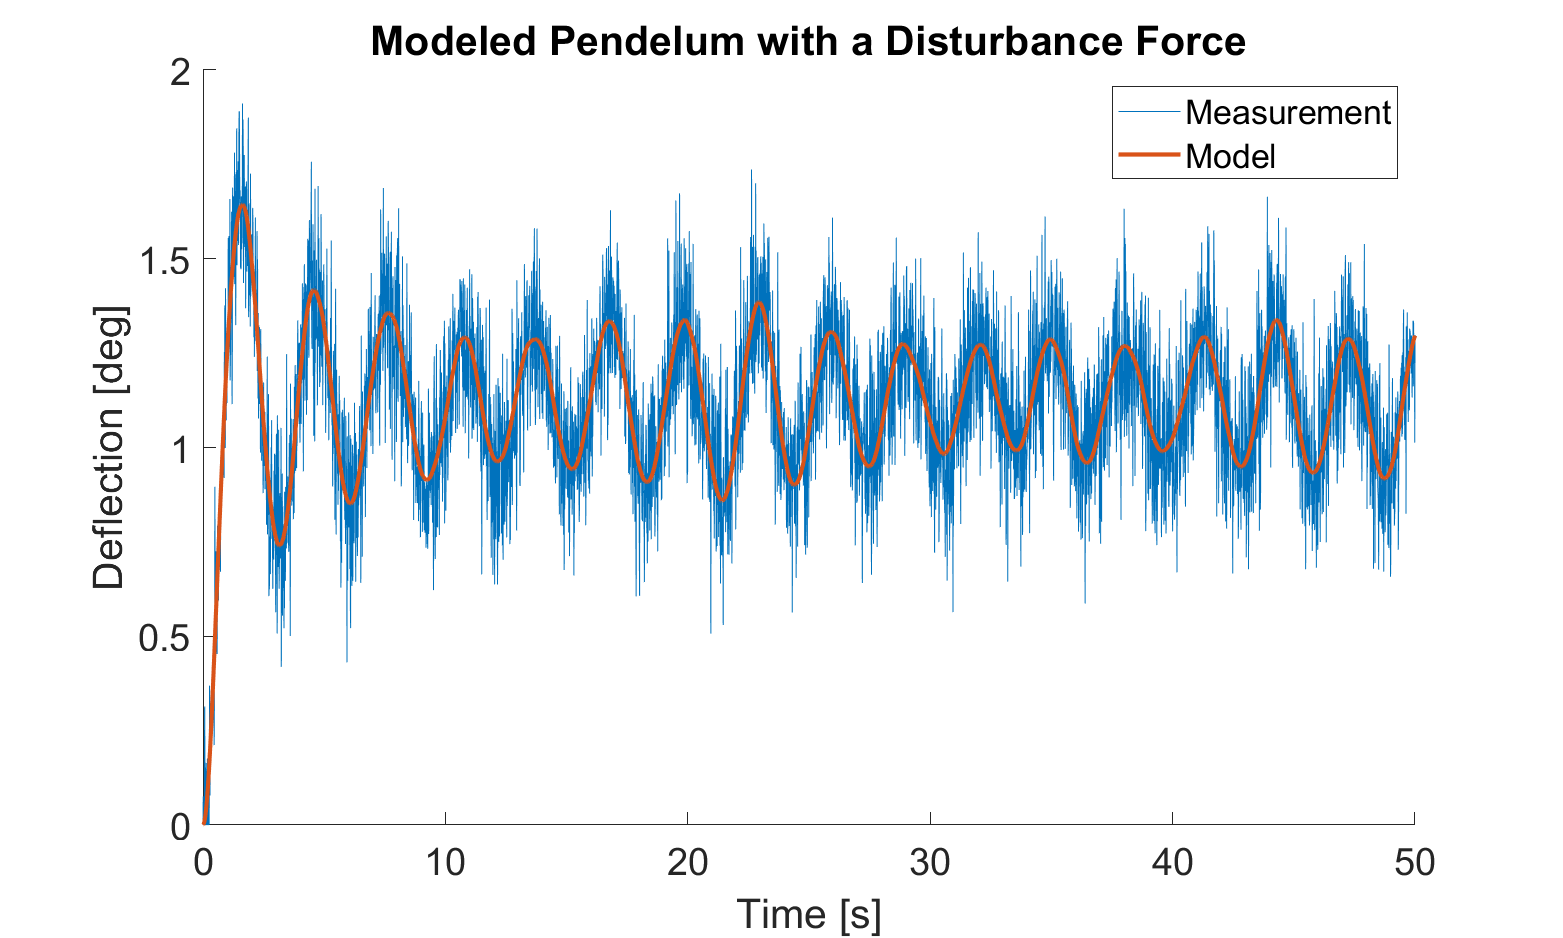
\includegraphics[width=0.7\linewidth]{Q1model.png}
                \caption{Modeled pendulum and the measurement of deflection through time}
                \label{fig:1}
            \end{figure}
        }
        We can model the pendulum by writing the angular acceleration,$\ddot{\theta}$, as a second-order ODE (Equation \ref{eq:1}). I assume small angle approximation based on my smaller time step.
        \begin{equation}
            \begin{split}
                \ddot{\theta} & = \frac{\tau}{J_p} + \frac{f_{d}L\theta}{J_p} - \frac{mgL\theta}{Jp} - \frac{b\dot{\theta}^3}{Jp}
            \end{split}
            \label{eq:1}
        \end{equation}
        To get $\dot{\theta}$ and $\theta$ we can integrate once, and then integrate again, respectively.
        \clearpage
        \part{Develop an extended Kalman filter to estimate the position and velocity (and any additional needed parameters) of the pendulum given measurements as described.}

        \part{Develop an unscented Kalman filter to estimate the position and velocity (and any additional needed parameters) of the pendulum given measurements as described.}

        \part{Use Monte Carlo simulations to compare the performance of the EFK and UKF. Be sure to compare expected covariance to sampled covariance from Monte Carlo simulations.}
    \end{parts}

    \question{Refer to problem 3 from homework \#3 (the 'Navigation' filter). Design a particle filter to estimate the East and North position, radar, and gyro bias using the data (\textbf{hw3\_3} from canvas). Compare the performance of the particle filter to the performance of your estimator from homework \#3 using at least 3 different numbers of particles. ($N = 50, 100, 1000$). Provide plots of estimations error, analytical covariance (from EKF) and numerical covariance (from particle filter).}
\end{questions}

\end{document}